\documentclass[uplatex, titlepage, report]{jsbook}

%%%%%%%%%%%%%%%%%%%%%%%%%%%%%%%%%%%%%%%%%%%%%%%%%%%%
% パッケージはここに追加。
%1行目に何に使うか、2行目以降に使い方をコメントすること。
%%%%%%%%%%%%%%%%%%%%%%%%%%%%%%%%%%%%%%%%%%%%%%%%%%%%

%一括コメントアウト
%\begin{comment}
\usepackage{comment}

%数学記号
%多数あるが、例えば\thereforeで'∴'(ゆえに)が出せる。
\usepackage{amssymb}

%行列、ベクトルなど
%\begin{pmatrix}…\end{pmatrix}。表と同じように区切り、改行する。縦ベクトルは1列の行列として表現。
\usepackage{amsmath}

%定理・補題・定義・証明
%\begin{theorem}, \begin{lemma}, \begin{definition}, \begin{proof}
\usepackage{amsthm}

%ブラケット記法
%\bra{a}, \ket{a}, \braket{a|H|a}。先頭を大文字にする(\Bra, \Ket, ...)と、
%中身の大きさに応じてブラケットの大きさも変わる。
\usepackage{braket}

%フォントの変更
%なし(自動)。
\usepackage{newpxtext, newpxmath}

%画像の挿入
%\includegraphics[width=***cm]{***.pdf}
\usepackage[dvipdfmx]{graphicx}

%文章を四角で囲む/左に線を引く
%\begin{oframed}、\begin{leftbar}など。
\usepackage{framed}

%図表を強制的にその場所に配置
%位置指定で[h]のかわりに[H]とする。これを使うと行間が不自然になる場合もある。
\usepackage{here}

%文字の色を変える
%\textcolor{red}{text}など。
\usepackage{color}

%urlをそのまま記載できる
%\url{http://www.....}
\usepackage{url}

%urlやページへのリンク
%なし(自動)。
\usepackage[
    dvipdfmx,
    bookmarkstype=toc,
    setpagesize=false,
    colorlinks=true,
    urlcolor=black,
    linkcolor=black,
    citecolor=black,
    bookmarks=true,
    bookmarksopen=true,
    bookmarksnumbered=true]{hyperref}
    
%urlやページへのリンク(hyperrefを日本語環境で使用するのに必要)
%なし(自動)。
\usepackage{pxjahyper}

%著者をまとめて表示
%省略(rootでしか使用しないため)。
\usepackage{authblk}

%花文字
%\mathscr{A}
\usepackage{mathrsfs}

%化学式
%\ce{^3He},\ce{Na2SO3}
\usepackage[version=3]{mhchem}

%%%%%%%%%%%%%%%%%%%%%%%%%%%%%%%%%%%%%%%%%%%%%%%%%%%%
%マクロはここに追加。
%1行目に何に使うか、2行目以降に使い方をコメントすること。
%文書全体で使用するマクロのみここで定義。自分だけ使用する場合は、
%自分の文書を\begingroup - \endgroupもしくは{ }で囲み、その中で定義
%する。
%%%%%%%%%%%%%%%%%%%%%%%%%%%%%%%%%%%%%%%%%%%%%%%%%%%%

%等号の上下に文字列を表示。文字列の長さに応じて等号が伸縮。
%\xequal[下]{上}
\makeatletter
\newcommand{\xequal}[2][]{\ext@arrow 0055{\equalfill@}{#1}{#2}}
\def\equalfill@{\arrowfill@\Relbar\Relbar\Relbar}
\makeatother

%%%%%%%%%%%%%%%%%%%%%%%%%%%%%%%%%%%%%%%%%%%%%%%%%%%%
%スタイルの変更はここに追加。
%1行目に変更するスタイルをコメントすること。
%%%%%%%%%%%%%%%%%%%%%%%%%%%%%%%%%%%%%%%%%%%%%%%%%%%%
%脚注
\renewcommand{\thefootnote}{\arabic{footnote})}

%定理環境(amsthm)
\theoremstyle{definition}
\newtheorem{theorem}{定理}
\newtheorem{definition}[theorem]{定義}
\newtheorem{lemma}[theorem]{補題}
\renewcommand\proofname{\textbf{証明}}

%著者
\renewcommand\Authsep{\quad}
\renewcommand\Authands{\quad}

%もう少しまともなタイトルを考える
\title{スピン・エコー}

\date{\vspace{3cm} 
\includegraphics{logo.pdf}\\ \vspace{5cm} 提出年月\quad2017年4月}

\author[$\dagger$]{加須屋春樹}
\author[$\dagger$]{近藤寛記}
\author[$\dagger$]{鈴木一輝}
\author[$\dagger$]{武中亮}
\author[$\dagger$]{間宮章}
\author[$\dagger$]{藤井涼平}
%Bad practiceだが、こうするくらいしか思いつかない
\author[ ]{\\}

\affil[$\dagger$]{京都大学 理学部}
\author[ ]{\\}
\author[ ]{指導教員\quad}
\author[*]{菅沼秀夫 准教授}
\author[*]{成木恵 准教授}
\affil[*]{京都大学 理学研究科}
\begin{document}
\maketitle
\tableofcontents

%ここで文書をincludeします
\section{スーパーミラーによるスピンの選択}
\nocite{neutron_spin_optics}
この実験では、特定のスピンを持つ中性子を選択的に取り出す必要がある。この節では、そのために用いるスーパーミラーの原理について説明する。

\subsection{中性子の光学的性質}
\paragraph{屈折率}
中性子が物質中で感じるポテンシャルを$V$とすると、エネルギー保存から
\begin{align}
k^2-k'^2=2mV
\end{align}
となる。$k$は入射中性子の波数、$k'$は物質中での中性子の波数である。
屈折率の定義
\begin{align}
n=\frac{k'}{k}
\end{align}
から、中性子の物質中における屈折率は
\begin{align}
n^2=1-\frac{2mV}{k^2}\label{mirror_neutron_refindex}
\end{align}
となる。

\paragraph{全反射が起きる条件}\label{mirrir_perfect_reflection}
$n-1$が有限の値を持つことは、中性子が全反射しうることを意味する。全反射が起きるための角度の条件は、
臨界角
\begin{align}
\theta^*=\arccos{n}
\end{align}
を用いて
\begin{align}
n\leq\cos\theta^* \label{mirror_refindex_range}
\end{align}
となる。また、全反射が起きるための入射エネルギー$E$の条件は、(\ref{mirror_neutron_refindex}), (\ref{mirror_refindex_range})より
\begin{align}
&n^2=1-\frac{2mV}{k^2}\leq\cos^2\theta^*\\
&E\sin^2\theta\leq E\sin^2\theta^*=\frac{k^2}{2m}\sin^2\theta^*\leq V
\end{align}
となる。すなわち、臨界角以下で入射する時、エネルギーの``ミラーに対し垂直な成分''が$V$よりも小さければ、
全反射が起きることがわかる。

\subsection{磁性体単層膜によるスピンの選択}
磁性体の単層膜を利用することで、特定のスピンを持つ中性子を選択的に取り出すことができる。
中性子が単層膜中で受けるポテンシャルは、核力によるポテンシャル$V_\mathrm{n}$、単層膜中の磁束密度$B$を用いて
\begin{align}
V^{\pm}&=V_\mathrm{n}\pm|\mu_\mathrm{n}|B
\end{align}
となる。$\mu_\mathrm{n}|B|$の符号とスピンの向きの対応は磁場の向きによって決まるが、ここでは上向きスピンのときに正になるものとする。
すなわち、上向きスピンの中性子は$V^+$、下向きスピンの中性子は$V^-$を感じる。

\ref{mirrir_perfect_reflection}節で述べたように、入射中性子のエネルギーを$E$とすると、
\[
E\sin^2\theta\leq V
\]
のときに全反射が起きる。
$V^-< E\sin^2\theta\leq V^+$のエネルギーを持つ中性子をこの単層膜に入射させると、下向きスピンの中性子はほとんどが透過するが、
上向きスピンの中性子は全反射される。$V^+<E\sin^2\theta$の中性子が入射した場合は、上向き、下向き両方の粒子が
透過する確率を持つ。
そのため、透過した中性子には上向きスピンと下向きスピンの両方が含まれる。
$E\sin^2\theta\leq V^-$となるような低エネルギーの中性子は今回の実験では無視できるほど少ないため、
考えなくて良い。

\begin{figure}[h]
\centering
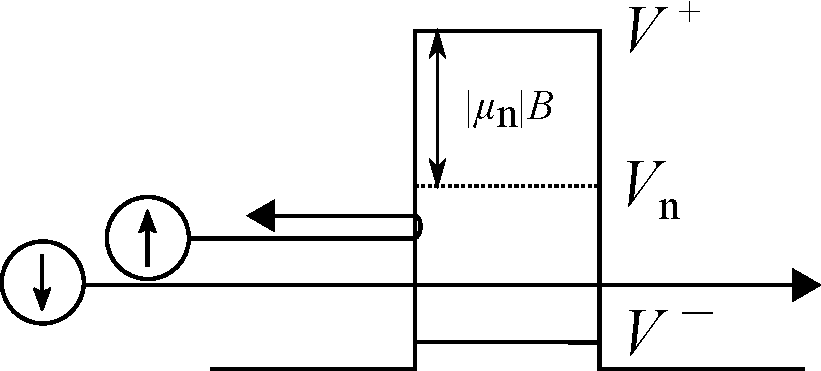
\includegraphics[width=8cm]{mirror/mono_mirror.pdf}
\caption{単層膜によるスピンの選択の原理。実際には、ポテンシャルは紙面奥に向かって2次元に広がっており、
中性子は臨界角以下で入射していることに注意。}
\end{figure}
このようにして、単層膜は上向きスピンの粒子のみを選択的に反射する。

\subsection{スーパーミラー}
\begin{figure}[H]
\centering
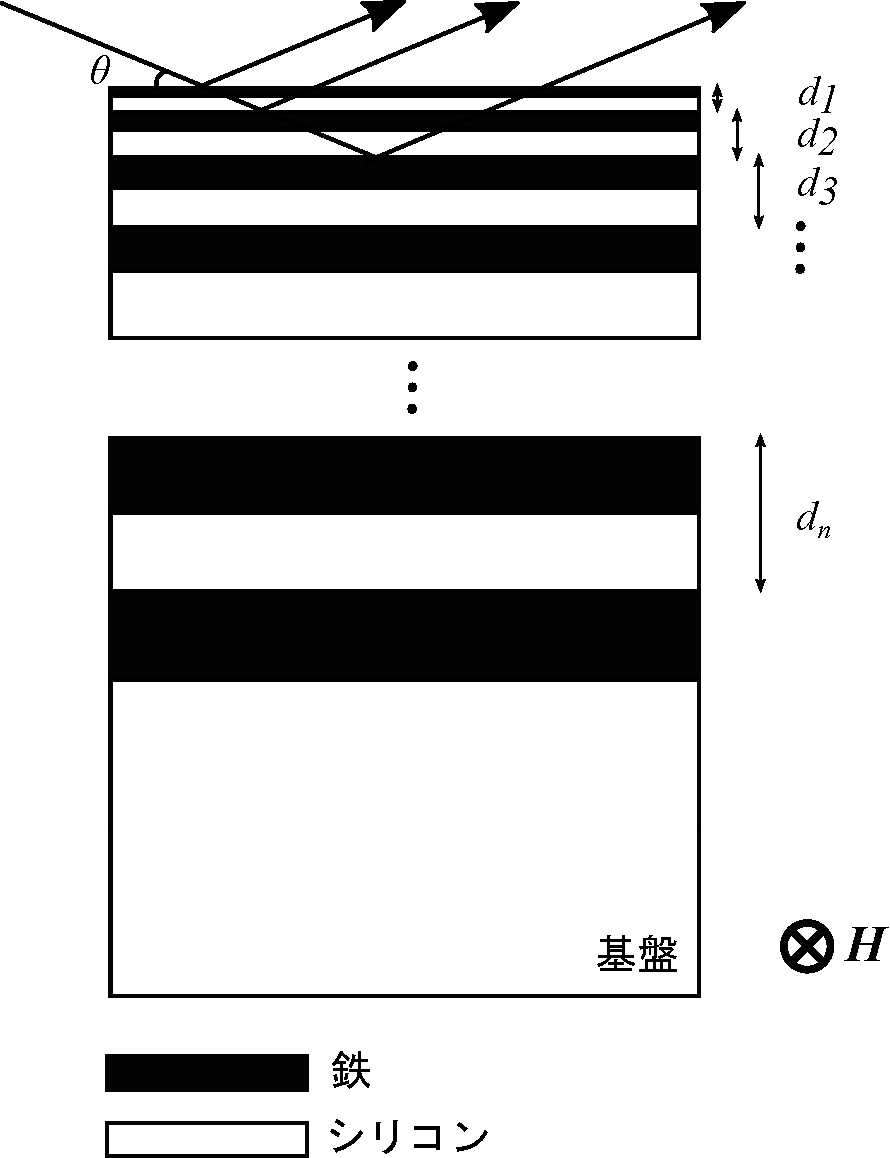
\includegraphics{mirror/super_mirror.pdf}
\caption{スーパーミラーの構造\cite{seki}\label{mirror_super_mirror}}
\end{figure}
\begin{figure}[h]
\centering
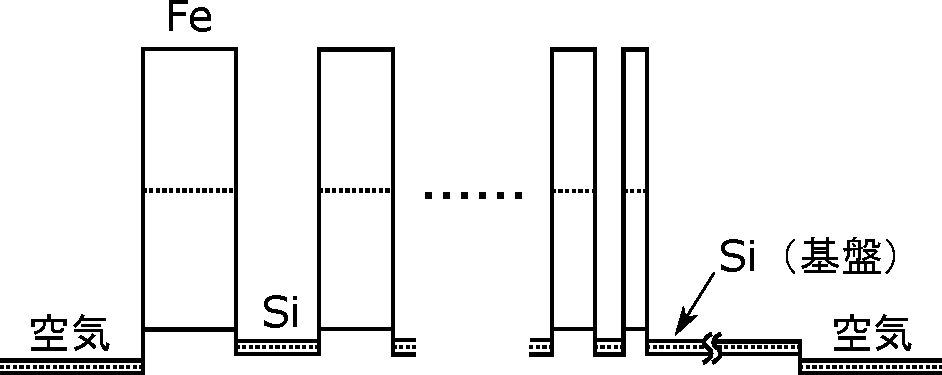
\includegraphics[width=9cm]{mirror/super_mirror_potential.pdf}
\caption{スーパーミラーのポテンシャル。破線は磁場によらない核力によるポテンシャル。実線(上)は上向きスピンの中性子が感じるポテンシャル。
実線(下)は下向きスピンの中性子が感じるポテンシャル。空気やシリコンの透磁率は小さいため、全体に磁場をかけても
ポテンシャルはほとんど影響を受けない。}
\end{figure}
図\ref{mirror_super_mirror}のように膜厚を少しずつ変えた多層膜を使うことで、
単層膜よりも高いエネルギーの中性子を反射するミラーを作ることができる。
これをスーパーミラーと呼ぶ。

\paragraph{Bragg反射による偏極}
$E\sin^2\theta\leq V^+$の中性子は多層膜の表面で全反射されるが、$V^+<E\sin^2\theta$の中性子は多層膜の内部に侵入する。
多層膜の膜間隔を$d$とすると、侵入した中性子はBragg条件
\begin{align}
2d\sin\theta=\lambda
\end{align}
を満たす場合に反射波が強め合う。$\lambda$は中性子の物質波の波長で、
$\lambda=2\pi/k$の関係にある。

$d$を少しずつ変えることで、$V^+<E\sin^2\theta$の様々なエネルギーを持つ上向きスピンの中性子がBragg反射される。
下向きスピンの中性子もわずかに反射されるが、その数は少なく、無視できる。
こうすることで、単層膜に比べより広いエネルギーの中性子のスピンを偏極することができる。

\section{検出器}
中性子は電荷をもたないため、その検出は強い相互作用を通じて行われる。強い相互作用による反応で生じた荷電粒子を検出することで、間接的に中性子を検出する。検出に利用する反応は検出する中性子のエネルギーによって様々であるが、熱中性子($\sim 25$ meV)の場合、次のような中性子捕獲反応が主に利用される:
\begin{align}
&\ce{^3He} + \ce{n} \to \ce{^3H}+\ce{p} + 0.705 \mathrm{MeV} \label{Kasuya_3He} \\
&\ce{^6Li} + \ce{n} \to \ce{^3H}+\ce{^4He}+4.78 \mathrm{MeV} \label{Kasuya_6Li}
\end{align}

\subsection{$\ce{^3He}$ガスを充填した比例計数管}
今回の実験では入射する中性子の時間情報と個数を知る必要がある。そこで入射粒子の数を1つずつ数える微分型の検出器として、$\ce{^3He}$ガスを充填した比例計数管を用いた。

\paragraph{検出原理}
検出には(\ref{Kasuya_3He})の反応が利用される。反応で生じた荷電粒子が気体中を進むと、軌道上の気体分子が電離してイオン・電子対が生じる。電場をかけてそれらを集めることで、信号として読み取ることができる。エネルギー25meVの中性子に対する$\ce{^3He}$原子核の断面積は$5333$barn[]であり、低エネルギーでこの断面積は中性子の速度に反比例することが知られている[]ため、エネルギー$E$(meV)の中性子に対する$\ce{^3He}$原子核の断面積は$\sigma(E)=5333\sqrt{25/E}$(barn)となる。これは気体の中では非常に大きく、効率よく中性子の数を数えることができる。

\paragraph{検出器の仕組み}
円筒形の容器の中に$\ce{^3He}$ガスが封入されており、高電圧がかけられた中心のワイヤと接地された容器の内壁がそれぞれ陽極と陰極として機能する。$\ce{^3He}$ガスは(\ref{Kasuya_3He})の反応によって荷電粒子を発生させる中性子有感物質であると共に、この荷電粒子によって電離して信号を増幅させる被電離気体の役割を果たす。

\begin{figure}[h]
\begin{minipage}{0.5\hsize}
\begin{center}
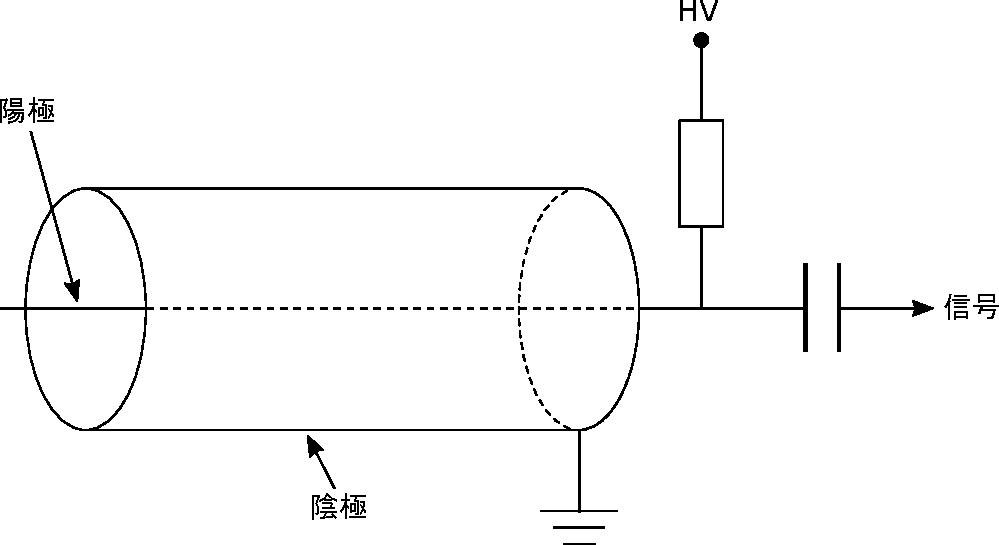
\includegraphics[width=6.5cm]{detector/detector_fig1.pdf}
\caption{比例計数管写真}
\end{center}
\end{minipage}
\begin{minipage}{0.5\hsize}
\begin{center}
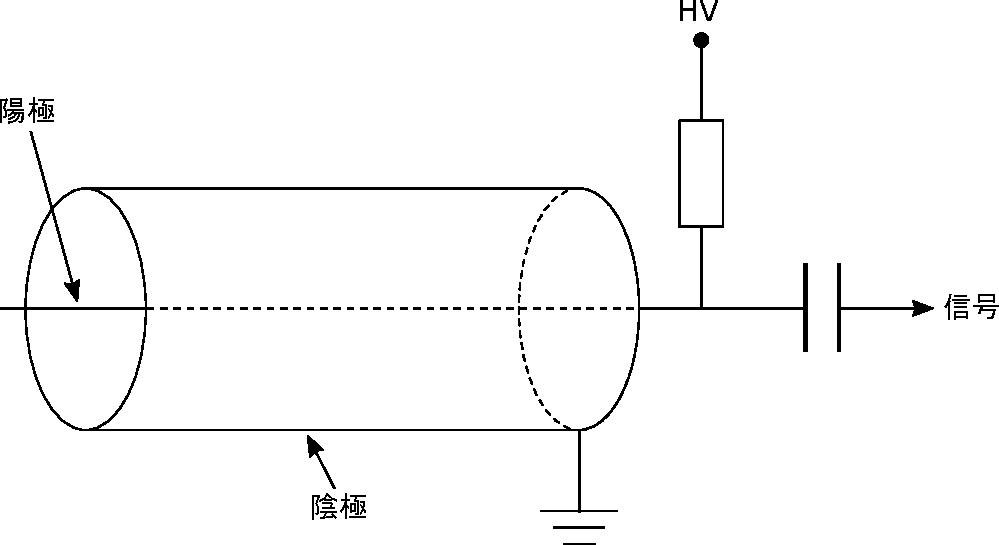
\includegraphics[width=6.5cm]{detector/detector_fig1.pdf}
\caption{比例計数管模式図}
\end{center}
\end{minipage}
\end{figure}

\subsection{RPMT検出器}
予備実験では入射する中性子の2次元的な位置情報を知る必要がある。そこで2次元位置感度型検出器として、RPMT検出器を用いた。

\paragraph{検出原理}
検出には(\ref{Kasuya_6Li})の反応が利用される。反応で生じた荷電粒子によってシンチレータ中の原子や分子が励起され、下の準位に戻る際に光が放出される(シンチレーション光)。生じた光は光電子増倍管で増幅され信号として取り出される。RPMTではシンチレータに$\ce{^6LiF}/\ce{ZnS}$を用いる。$\ce{^6LiF}/\ce{ZnS}$は発光量が大きくガンマ線感度が低いことから、中性子の検出に適している。

\paragraph{検出器の仕組み}
RPMTは$\ce{^6LiF}/\ce{ZnS}$シンチレータにPSPMT(Position Sensitive PMT,位置分解能をもつ光電子増倍管)を取り付けた構造をしている。PSPMTは内部にX軸Y軸のメッシュ状の読み取り用電極をもち、電荷分割法により中性子の検出位置を$x/L=Q_2/(Q_1+Q_2)$で求めることができる。ここで$L$は電極の全長、$x$は検出位置、$Q_1,Q_2$は2本のケーブルからの出力電荷である。検出位置はX軸Y軸について1024ch$\times$1024chの分解能で計測され、チャンネル幅[mm/ch]は$1\mathrm{[ch]}=0.119\pm0.002\mathrm{[mm]}$と報告されている[]。

\begin{figure}[h]
\begin{minipage}{0.5\hsize}
\begin{center}
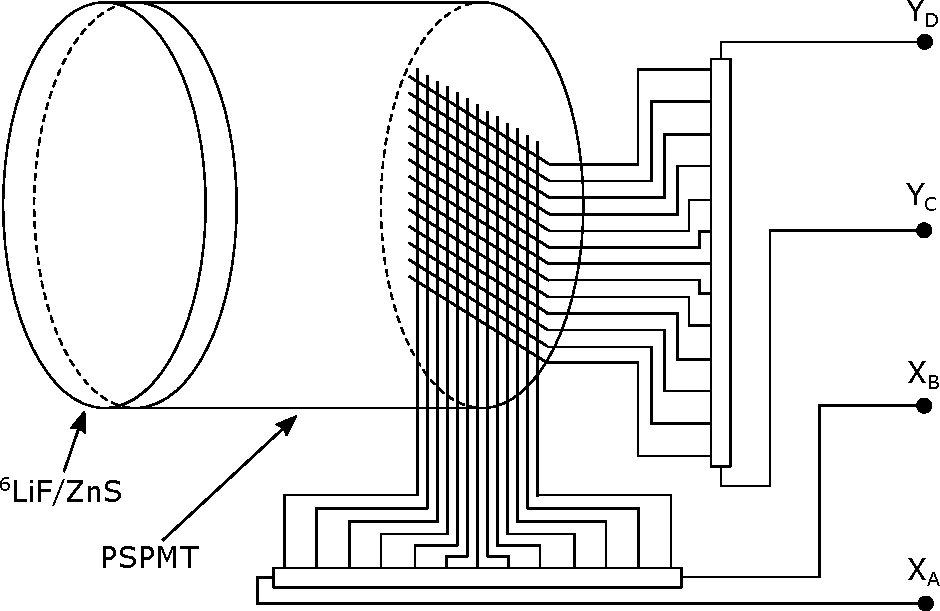
\includegraphics[width=6.5cm]{detector/detector_fig2.pdf}
\caption{RPMT写真}
\end{center}
\end{minipage}
\begin{minipage}{0.5\hsize}
\begin{center}
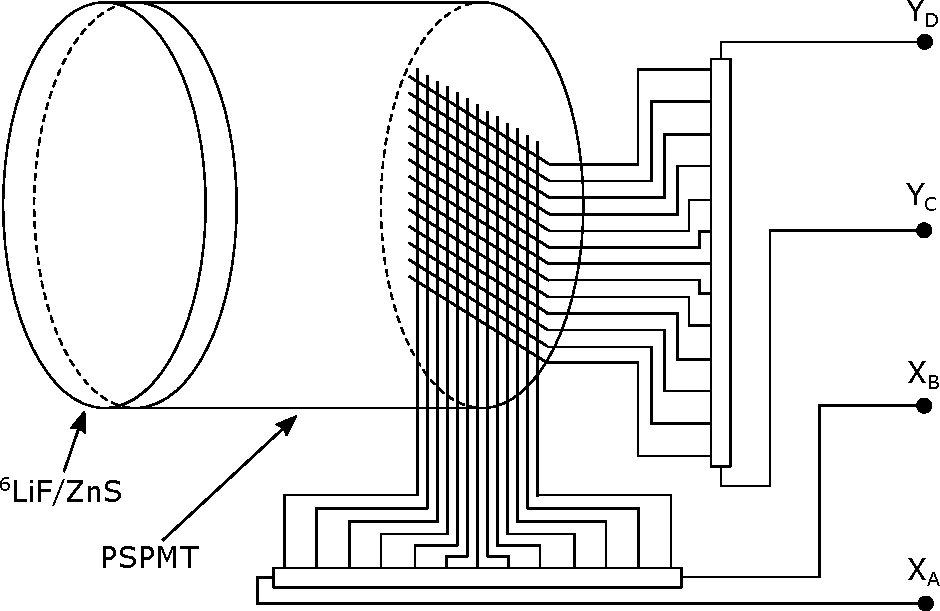
\includegraphics[width=6.5cm]{detector/detector_fig2.pdf}
\caption{RPMT模式図}
\end{center}
\end{minipage}\\
\begin{minipage}{0.5\hsize}
\begin{center}
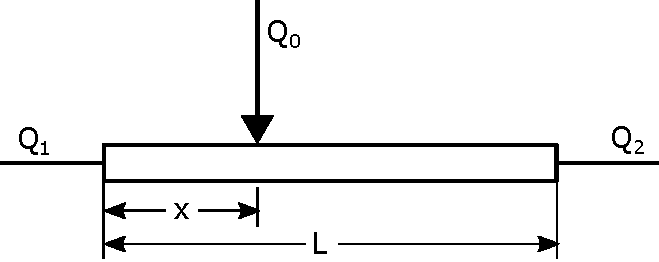
\includegraphics[width=6.5cm]{detector/detector_fig3.pdf}
\caption{電荷分割法}
\end{center}
\end{minipage}
\end{figure}







\bibliographystyle{jplain}
\bibliography{bibliography}
\end{document}
